\clearpage
\section{Useful MATLAB Functions}

\underline{\textbf{Set up Transfer Function}}

Given transfer function in s-domain
    \begin{equation*}
        G = \frac{s-3}{(s+1)(s+2)} = \frac{s-3}{s^2+3s+2}
    \end{equation*}

\begin{lstlisting}
% Approach 1
s = tf('s');
Gs = (s-3) / ( (s+1) * (s+2) );
% Approach 2
num = [1 -3];
den = [1 3 2];
Gs = tf(num,den);
% Approach 3
num = [1 03];
den = conv([1 1],[1 2]);
Gs = tf(num,den);
%% If in z-domain ...
T = -1;
z = tf('z', T);  % T=-1 means sampling time
                 % unspecified
% rest are similar
\end{lstlisting}

Given pole locations as
\begin{equation*}
    z_{1,2} = 1.87 \pm j\, 1.36
\end{equation*}

\begin{lstlisting}
z1 = 1.87 + 1i * 1.36; 
z2 = 1.87 - 1i * 1.36;
den = poly([z1,z2])
>> den = 1.0000   -3.7400    5.3465
\end{lstlisting}

Given plant transfer function in s-domain and sampling time, find ZAS:
\begin{equation*}
    \text{Given } \begin{cases}
    G_p(s) = \frac{1}{s(s+1)} \\
    T = 0.04 \; \text{sec}
    \end{cases}
\end{equation*}
\begin{lstlisting}
num_c = [1];
den_c = [1 1 0];
T = 0.04;  % cannot set to -1 for 
           % unspecified case
[num_d den_d] = c2dm(num_c,den_c,T,'zoh');
Gp_zas = tf(num_d,den_d,T)
\end{lstlisting}

Given CE as follow, find roots.
\begin{equation*}
    \text{CE} = \frac{9/8}{z^2+1.5z+9/8}
\end{equation*}
\begin{lstlisting}
CE = tf([9/8], [1 1.5 9/8], -1); % T=-1
zeors = roots(cell2mat(CE.Num));
poles = roots(cell2mat(CE.Den))
>> poles =
  -0.7500 + 0.7500i
  -0.7500 - 0.7500i
\end{lstlisting}



\textbf{\underline{Other Minutiae:}}
\begin{itemize}
    \item Instantaneous Gain: \textbf{Wolfram Alpha}.
    \item DC Gain:
\end{itemize}
\begin{lstlisting}
% Case 1: in s-domain
dcgain(sys_s);
% Case 2: in z-domain
evalfr(sys_z, 1) % since G(1) = DC. G.
\end{lstlisting}

\begin{itemize}
    \item Partial fraction decomposition:
    \begin{align*}
        \text{Given that }\; \frac{-4s+8}{s^2+6s+8} \\
        \text{want: }\, \frac{-12}{s-(-4)} + \frac{8}{s-(-2)}
    \end{align*}
\end{itemize}
\begin{lstlisting}
num = [-4 8];
den = [1 6 8];
[r p k] = residue(num,den)
>> r = [-12 
          8]
>> p = [-4 
        -2]
>> k = []        
\end{lstlisting}


\textbf{\underline{Transformation Summary}}
\begin{figure}[h]
    \centering
    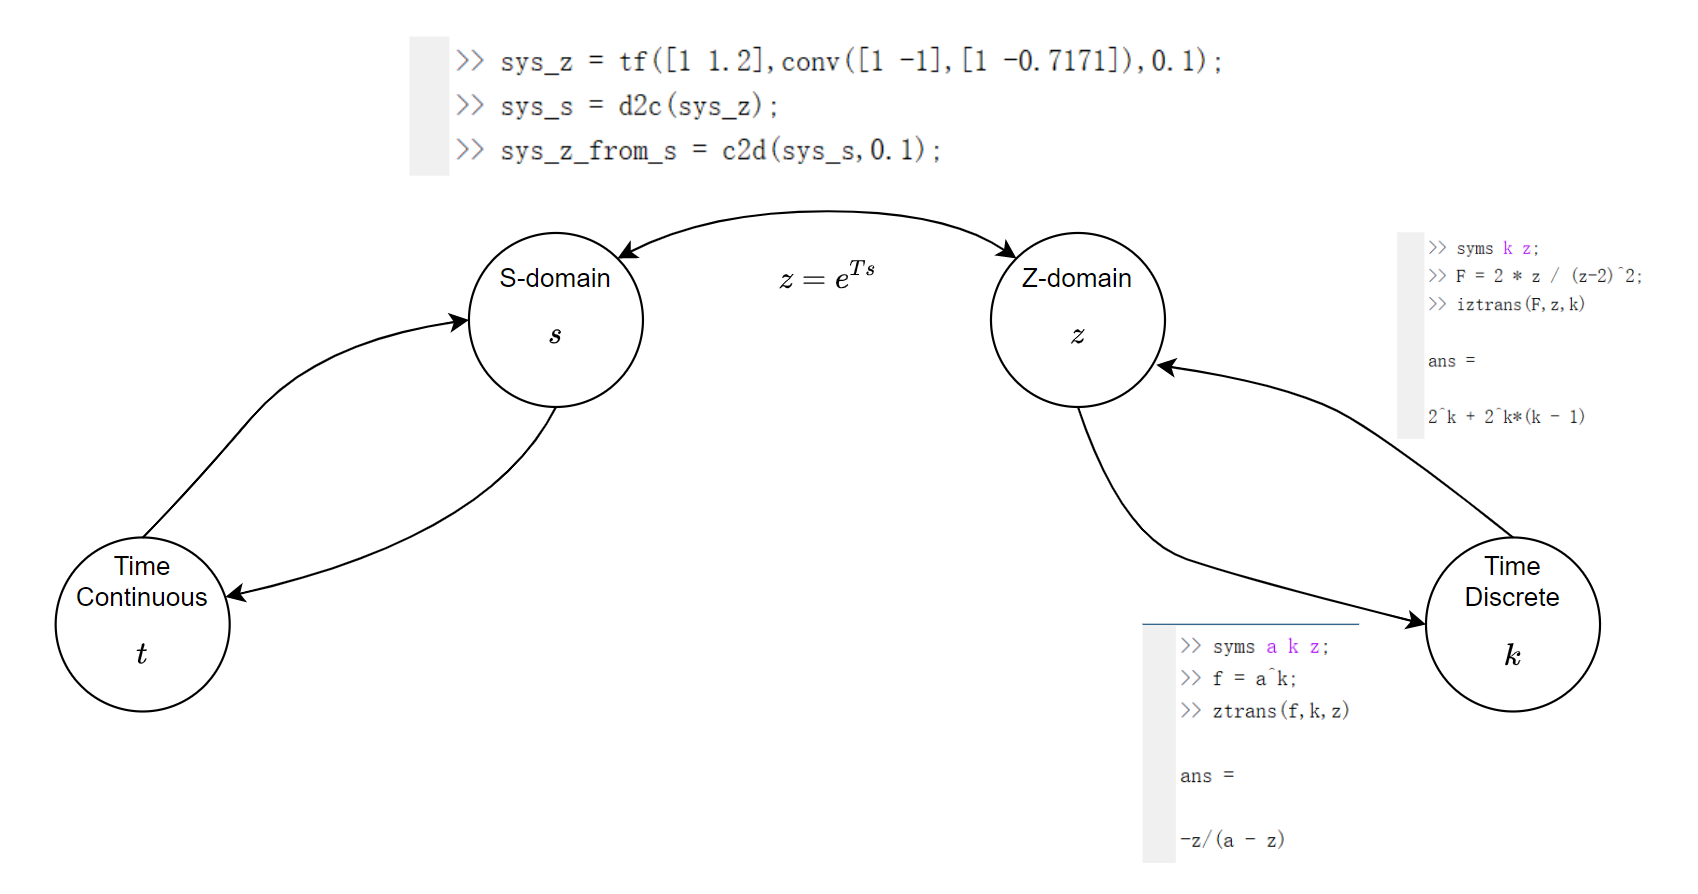
\includegraphics[width=1.0\linewidth]{images/transformation_Summary.png}
\end{figure}